\documentclass[10pt]{article}
\usepackage[preprint]{tmlr}

\usepackage{microtype,amsmath,amssymb,amsthm,booktabs,graphicx,array}
\usepackage[colorlinks=true,allcolors=blue]{hyperref}
\usepackage{url}
\hypersetup{pdftitle={CAEA: Auditing and Repairing Preference-Induced Belief Feedback},pdfauthor={Xiaotong Zhang}}

\usepackage{enumitem}
\setlist{nosep,leftmargin=*}
\newtheorem{theorem}{Theorem}
\newtheorem{proposition}[theorem]{Proposition}
\newtheorem{corollary}[theorem]{Corollary}
\newcommand{\E}{\mathbb E}
\newcommand{\KL}{D_{\mathrm{KL}}}
\newcommand{\TV}{\operatorname{TV}}
\newcommand{\Var}{\operatorname{Var}}
\newcommand{\sig}{\operatorname{sigmoid}}
\title{CAEA: Auditing and Repairing Preference-Induced Belief Feedback}
\author{\name Xiaotong Zhang\\
\addr China University of Petroleum (East China)\\
Qingdao, China}

\date{}
\begin{document}
\maketitle

\begin{abstract}
Pooled single-turn evaluations can miss whether an assistant amplifies
belief differences over repeated interactions.
We demonstrate this gap in a controlled binary response model: increasing
agreement pressure leaves the entire pooled response--outcome distribution
unchanged, while the mean-response dynamics change from convergence to
separated stable beliefs. We study conflict-aware epistemic alignment
(CAEA), which repairs an externally audited content distribution while
retaining the preference policy within each content class. Classical KL
projection quantifies the preference cost; coupling bounds relate repair
strength to feedback contraction. Finite stance audits cannot certify
global stability without additional regularity; a known curvature bound
yields a finite-sample certificate. Ten-seed finite-action DPO experiments,
stochastic simulations, and two frozen-language-model candidate-selector
pilots illustrate these results and their limits. Full repair and audit-only
have identical forecast risk by construction. Soft-score reweighting can
achieve a better risk--KL tradeoff, and option permutations remove the
pilots' initial DPO gains. The contribution is an analysis of audit
observability, conditional repair, and stability under explicit assumptions;
it does not establish benefits for human cognition or free-text generation.
\end{abstract}


\section{Introduction}
An assistant can give acceptable answers in isolation yet reinforce a user's
unsupported belief over repeated exchanges. Human preference judgments can
reward agreement at the expense of truthfulness \citep{sharma2024}, creating
a plausible mechanism for such feedback. The mechanism is conditional:
agreement can be warranted, and preference optimization can also reward
evidence-based correction. The relevant question is therefore when
preference adaptation changes the stability of an interaction, rather than
whether preference alignment and epistemic quality are inherently incompatible.

Consider users who receive the same evidence but express different beliefs.
If an assistant responds to each user's unsupported stance, averaging its
answers across users may conceal systematic differences in what each user
receives. We formalize this distinction with a binary construction: the
pooled one-turn response--outcome distribution, including its Brier risk,
remains unchanged as agreement pressure increases, while the mean-response
interaction acquires separated stable equilibria. A pooled audit and a
feedback analysis can therefore give different answers about the same policy.

We study a corresponding intervention, conflict-aware epistemic alignment
(CAEA). An external audit partitions responses into epistemic classes and
specifies a target distribution over those classes. CAEA changes the class
marginal while retaining the preference policy conditional on each class.
This permits a precise distinction between changing an answer's audited
content and changing its remaining attributes. In the experiments, classes
encode probability reports and within-class variation encodes abstract style;
whether this partition captures all information affecting a human reader
is a separate empirical question.

The analysis connects three quantities: the epistemic marginal being
enforced, the preference cost of changing it, and the intervention strength
needed for a specified contraction margin. It also identifies what an audit
must assume. Finite observations at selected stances cannot certify global
stability for an unrestricted smooth response function; a supplied curvature
bound makes a conservative finite-sample certificate possible.

\paragraph{Contributions.}
The central result is a counterexample to identifying feedback stability
from a pooled one-turn joint distribution, not a claim that preference
optimization is universally harmful. We connect this observability gap to
(i) an exact repair threshold in the binary mean-response model,
(ii) preference-cost accounting and contraction bounds for conditional
repair, and (iii) a finite-audit impossibility result and a certificate
conditional on supplied regularity. The KL projection itself is classical,
and closest-KL anti-sycophancy correction is prior work. Our analysis asks
what the audit observes, what intervention its target requires, and which
feedback guarantee follows. Controlled training and simulations test the
implementation and expose adverse baselines, auditor failure, and neural
selector transfer failures.

\begin{figure}[t]
\centering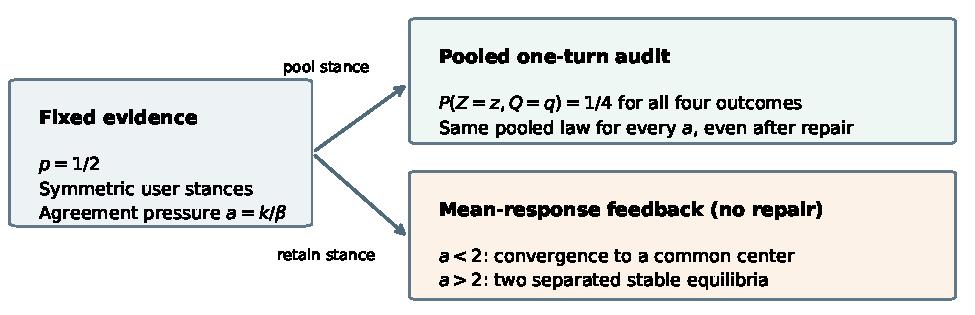
\includegraphics[width=\linewidth]{figures/audit_concept.pdf}
\caption{Two views of the same controlled binary model. Pooling over a
symmetric stance population hides agreement pressure; retaining stance
reveals different mean-response feedback regimes. The displayed threshold
uses zero repair. This is a model counterexample, not a claim about human
belief thresholds.}
\label{fig:concept}
\end{figure}

\section{Related work}
\paragraph{Preference optimization and sycophancy.}
DPO expresses preference learning through a policy/reference likelihood
ratio \citep{rafailov2023}. Empirical evidence links sycophancy to human
preference judgments \citep{sharma2024}. Shapira et al.\ analyze behavioral
amplification and derive a closest-KL correction that prevents increased
agreement \citep{shapira2026}; their result is the closest antecedent to our
projection component. Our emphasis is the connection between a class-marginal
repair and longitudinal feedback, including the observability limits of
pooled and finite stance audits. Moya et al.\ identify spurious-learning
mechanisms and a tie-training intervention \citep{moya2026}, highlighting
that confirmation-biased labels are not the only source of undesirable drift.

\paragraph{Belief updating and multiple perspectives.}
BASIL distinguishes sycophantic shifts from Bayesian updating and studies
calibration and post-training \citep{atwell2026}. Ma et al.\ separate
unsupported yielding from rational updating \citep{ma2026}; PlurPO constructs
preferences using multiple stakeholder perspectives \citep{hatgis2026}.
These approaches motivate evaluating selectivity rather than suppressing
agreement indiscriminately. Our evidence-fixed intervention changes a
user's unsupported stated stance, while informative user input belongs in
the evidence. Ghosh et al.\ investigate nonlinear belief dynamics under
sycophantic feedback \citep{ghosh2026}. We focus on a response-policy
construction with explicit audit equivalence and repair-budget calculations.

\paragraph{Projection, scoring, and diversity.}
The repair follows from the KL chain rule and information projection
\citep{csiszar1975}. Forecast evaluation uses proper-score regret
\citep{gneiting2007}. Output-diversity methods such as DivPO
\citep{lanchantin2025} address a different property: a broad distribution of
answers need not be well calibrated. We use standard statistical quantities
to keep these distinctions explicit.


\section{Problem formulation}
Let $x$ denote shared admissible evidence and $s\in[0,1]$ a user's stated
probability. Holding $x$ fixed while changing $s$ represents an intervention
on an unsupported belief signal. Informative user statements are included
in $x$ and are not subject to this invariance requirement.

The response space $\mathcal Y$ is finite. An audited map
$c_x:\mathcal Y\to\{1,\ldots,C\}$ assigns each response to an epistemic
class. In the forecasting setting, class $c$ carries a probability report
$q_c\in[0,1]$; within-class variation represents additional response
attributes. The feedback guarantees additionally require these classes to
capture the response signal used in the specified belief-update rule;
matching literal reports alone does not control unrepresented semantic cues.
Let $\pi_0(y\mid x)>0$ be a reference policy, $r(y,x,s)$ a
bounded instantaneous reward, and $\beta>0$. Define
\begin{equation}
 J_{x,s}(\pi)=\E_\pi r(Y,x,s)-\beta\KL(\pi\|\pi_0),\qquad
 \pi_P(y\mid x,s)=\frac{\pi_0(y\mid x)e^{r(y,x,s)/\beta}}{Z_{x,s}}.
 \label{eq:gibbs}
\end{equation}
The Gibbs policy $\pi_P$ is the ideal distributional maximizer. Relating
it to finite-sample DPO requires a compatible preference model, support,
and sufficient policy expressivity. Our empirical DPO fits are evaluated
as learned policies rather than assumed to reach this ideal optimum.

Write $m_P(c\mid x,s)=\sum_{y:c_x(y)=c}\pi_P(y\mid x,s)$.
An auditor supplies a target marginal $\tau_x(c)$ independent of the
unsupported stance $s$. The auditor and the class map are inputs to CAEA.
In the controlled experiments, the Bernoulli evidence probability $p_x$
is known, and the target is
\begin{equation}
 \tau_x(c)\propto\exp\{-(q_c-p_x)^2/T_E\},\qquad T_E>0.
 \label{eq:target}
\end{equation}
Here $T_E$ is a chosen exploration tolerance. Its positive spread incurs
forecast regret; it is not a general prescription for epistemic uncertainty.
Strong evidence can justify a concentrated target. Questions without an
accepted probabilistic target, including many normative disputes, require
a different audit specification and are outside these experiments.


\section{Conditional epistemic repair}
For a repair fraction $\lambda\in[0,1]$, set
\begin{equation}
 b_\lambda=(1-\lambda)m_P+\lambda\tau_x,\qquad
 \pi_\lambda(y\mid x,s)=b_\lambda(c_x(y)\mid x,s)
                \pi_P(y\mid c_x(y),x,s).
 \label{eq:repair}
\end{equation}
Full repair ($\lambda=1$) replaces the epistemic marginal with the
stance-independent target. Partial repair interpolates between this target
and the preference marginal. Both preserve every positive-mass
class-conditional response distribution exactly.

\begin{proposition}[KL projection and preference cost]
\label{prop:projection}
For fixed $(x,s)$ and a target marginal $b$ supported by $m_P$, the policy
$\pi_b(y)=b(c_x(y))\pi_P(y\mid c_x(y))$ is the unique minimizer of
$\KL(\pi\|\pi_P)$ among policies with class marginal $b$. Moreover,
\begin{equation}
 J(\pi_P)-J(\pi_b)=\beta\KL(b\|m_P).
 \label{eq:cost}
\end{equation}
Full target matching and preference optimality coincide exactly when
$m_P=\tau_x$.
\end{proposition}

The proposition instantiates classical information projection
\citep{csiszar1975}. Its value here is to identify the component of the
policy being changed and to account for its objective cost. Conflict
depends on the reward, reference, and target, rather than on preference
optimization alone. Full proofs appear in Appendix~\ref{app:proofs}.

\paragraph{Response selection.}
After scoring a bank of $N$ candidates, normalize the preference scores
within each class, sample a class from $b_\lambda$, then sample a response
from its existing class-conditional distribution. The additional computation
is $O(N)$. Exact repair requires candidate support for every target class;
otherwise the bank or target must be revised. Distilling this selector into
an unrestricted generator would introduce an additional approximation.

\section{Feedback hidden by pooled evaluation}
We first isolate the distinction between pooled output quality and
stance-conditioned feedback in a binary response model.
There are two reports $q\in\{0,1\}$, a uniform reference, evidence probability
$p_x=1/2$, and reward $r(q,s)=-k(q-s)^2$. Let $a=k/\beta$. Then
\begin{equation}
 m_a(1\mid s)=\sig(a(2s-1)).
 \label{eq:binary}
\end{equation}
Under full repair, $\tau(1)=1/2$; under partial repair, the expected report is
$f_\lambda(s)=(1-\lambda)m_a(1\mid s)+\lambda/2$.

\begin{theorem}[Pooled audit blindness and a repair threshold]
\label{thm:blindness}
\textbf{Pooled observations.}
Let the population stance $S$ have a distribution symmetric about $1/2$.
Conditional on the fixed evidence, let $Z\sim\operatorname{Bernoulli}(1/2)$
be jointly independent of the stance and response-sampling randomness.
For every $a\ge0$ and every $\lambda$,
the pooled joint distribution of $(Z,q)$ is the same: both coordinates are
independent uniform binary variables. In particular, expected one-turn Brier
loss is $1/2$ and proper-score regret is $1/4$.

\textbf{Mean-response feedback.}
For the deterministic update
\begin{equation}
 s_{t+1}=F_\lambda(s_t)=(1-\eta)s_t+\eta f_\lambda(s_t),\quad0<\eta\le1,
 \label{eq:meanupdate}
\end{equation}
the derivative at $s=1/2$ is
$1-\eta+\eta(1-\lambda)a/2$. If $(1-\lambda)a<2$, $F_\lambda$ is a strict
global contraction. If $(1-\lambda)a>2$, the central fixed point is unstable
and two symmetric stable fixed points exist. Thus, the infimum repair fraction
for strict contraction along this mixture family is
$\lambda_{\rm crit}=\max\{0,1-2/a\}$ for $a>0$; equality at $(1-\lambda)a=2$
does not certify a geometric rate. For $a=0$, no repair is needed for stability.
\end{theorem}


Thus, tests based only on the pooled one-turn joint law cannot distinguish
the constructed feedback regimes. Conditioning on stance or retaining
linked longitudinal observations restores information that pooling discards.
The threshold characterizes this mean-response model; it is not an estimated
threshold for human interaction. The assistant policy is fixed throughout
the interaction rather than retrained after each round.

\begin{figure}[t]
\centering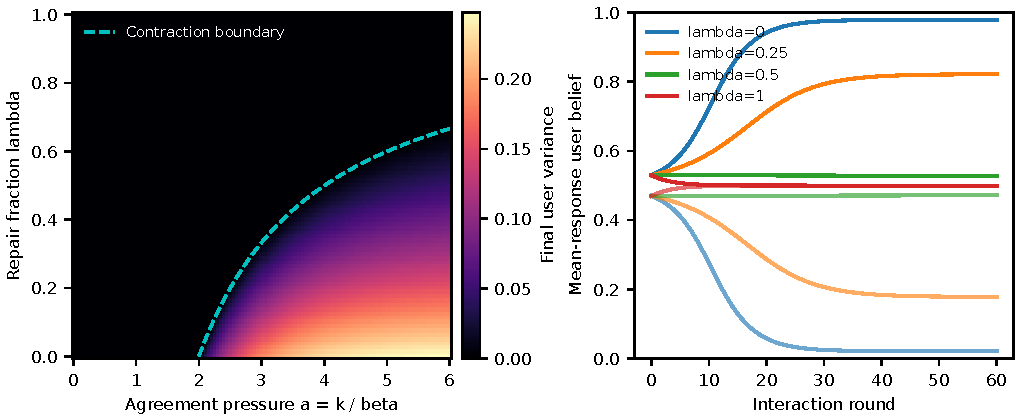
\includegraphics[width=.96\linewidth]{figures/phase.pdf}
\caption{Deterministic mean-response dynamics. Left: final
population variance after 400 updates from $s_0\in\{0.47,0.53\}$, $\eta=0.25$.
The dashed line is the strict-contraction boundary. Finite-horizon variance
remains nonzero near the boundary. Right: paired trajectories at $a=4$.
The simulations use the specified belief-update rule.}
\label{fig:phase}
\end{figure}

\section{Stability guarantees and audit requirements}
Let $K_{x,s}$ be the preference policy's distribution over report values $q_c$.
Assume a finite $L_x$ satisfies
$W_1(K_{x,u},K_{x,v})\le L_x|u-v|$, where $W_1$ is Wasserstein distance on
$[0,1]$. The same $\lambda_x$ must be used across non-evidential stances.
A stance-dependent repair fraction would introduce an additional feedback
term and requires a separate analysis.

\begin{theorem}[Stability budget and approximate full repair]
\label{thm:stability}
Fix $0<\eta\le1$. For the sampled update $U'=(1-\eta)U+\eta Q$,
the Markov kernel induced by
$K^\lambda_{x,s}=(1-\lambda_x)K_{x,s}+\lambda_x\tau_x$ is $W_1$-Lipschitz
with coefficient at most
\begin{equation}
 \rho_x=1-\eta+\eta(1-\lambda_x)L_x.
 \label{eq:rho}
\end{equation}
For a common evidence sequence with $\sup_x\rho_x<1$, differences between
initial belief distributions contract geometrically in $W_1$. This compares
belief laws, not the variance of independently sampled individuals.

Under full repair, suppose the implemented target $\widehat\tau_{x,s}$ differs
from a stance-independent ideal target by at most $\epsilon_t$ in total
variation at round $t$, uniformly over current belief states. Starting with the same initial belief and common
evidence, its belief law and the ideal target-driven law can be coupled so that
\begin{equation}
 \E|U_T-\widetilde U_T|
 \le\eta\sum_{t=0}^{T-1}(1-\eta)^{T-1-t}\epsilon_t.
 \label{eq:error}
\end{equation}
With a constant error bound, this is at most
$\epsilon[1-(1-\eta)^T]$.
\end{theorem}

If $L_x$ is known, a desired margin $\gamma\in(0,1)$ is obtained by choosing
$\lambda_x\ge\max\{0,1-(1-\gamma)/L_x\}$ for $L_x>0$, giving
$\rho_x\le1-\eta\gamma$. By convexity, $\KL(b_\lambda\|m_P)$ is
nondecreasing along $\lambda\in[0,1]$. Consequently, the smallest admissible
fraction minimizes the exact cost \emph{along this mixture path}; no
optimality over all stable policies is asserted. A positive margin avoids
the excluded boundary of a strict-contraction condition.

\begin{corollary}[A finite-audit expectation bound]
\label{cor:audit}
For $n\ge1$ independent class samples from a trusted target $\tau$ over $C$ classes,
the empirical frequency $\bar\tau$ satisfies
$\E\TV(\bar\tau,\tau)\le\tfrac12\sqrt{(C-1)/n}$.
For the add-$\alpha$ estimator
$\widehat\tau=(n\bar\tau+\alpha\boldsymbol1)/(n+C\alpha)$ with $\alpha\ge0$,
an upper bound is
\begin{equation}
 \E\TV(\widehat\tau,\tau)
 \le\min\left\{1,\frac12\sqrt{\frac{C-1}{n}}+
                   \frac{C\alpha}{n+C\alpha}\right\}.
 \label{eq:auditsamples}
\end{equation}
This controls target estimation error in expectation, not auditor bias.
\end{corollary}

\paragraph{Stability and correctness are distinct.}
An incorrect but stance-independent target can make the system stable and
wrong. Also, if unmeasured wording changes the interpreted epistemic signal,
the report-class map is not sufficient and Theorem~\ref{thm:stability} does not
cover that mechanism. Auditor validity and the sufficiency of the class
map are therefore separate requirements.

\subsection{From finite response audits to a stability certificate}
Equation~\eqref{eq:rho} requires a global sensitivity bound $L_x$.
Finite stance tests alone cannot establish it, even if the response
probability at every tested stance is known exactly.

\begin{proposition}[Finite stance audits need regularity]
\label{prop:finiteaudit}
For any finite set of audited stances $A\subset[0,1]$, there is a smooth,
bounded binary response probability $m(s)$ with $m(s)=1/2$ at every $s\in A$,
yet with two stable off-grid fixed points for
$F(s)=(1-\eta)s+\eta m(s)$, for every $0<\eta\le1$. Their separation can be
arbitrarily close to one. Thus, exact agreement with an invariant target on
finitely many stances cannot by itself certify global feedback stability.

Conversely, let $m\in C^2([0,1])$ satisfy a known global
curvature bound $|m''(s)|\le H$. Audit a uniform grid of $J\ge2$ points, spacing
$h=1/(J-1)$, with $n$ independent binary responses per point. Let
$\widehat m_j$ be the empirical means and
$\epsilon=\sqrt{\log(2J/\delta)/(2n)}$ for $0<\delta<1$.
With probability at least $1-\delta$,
\begin{equation}
 \sup_s|m'(s)|\le\widehat L_H:=
 \max_j\frac{|\widehat m_{j+1}-\widehat m_j|}{h}
       +\frac{2\epsilon}{h}+Hh.
 \label{eq:gridcertificate}
\end{equation}
This can be inserted into Equation~\eqref{eq:rho} for binary reports, where
the kernel $W_1$ distance equals the difference of response probabilities.
\end{proposition}

The $2\epsilon/h$ term penalizes overly fine grids at fixed observations per
point; $Hh$ penalizes overly coarse grids. For total report budget $N\simeq Jn$,
balancing the two errors gives $h$ of order $N^{-1/5}$ up to logarithms when
$H>0$ is fixed. A trustworthy curvature bound is additional information:
estimating it from the same unconstrained finite grid does not evade the first
part of the proposition. The certificate consequently trades sampling precision against coverage
under a supplied regularity assumption.

\section{Measuring report quality and belief dispersion}
We use three complementary quantities based on standard variance,
total-variation, and proper-scoring constructions. They describe different
objects: simulated belief dispersion, audited class coverage, and forecast
error. Their names do not imply validated measures of human cognition.

\paragraph{Belief Polarization Drift (BPD).}
For a common evidence context and matched initial user population, let
$V_T^\pi(x)=\Var(U_T^\pi\mid x)$ and let $\widetilde\pi$ use the trusted,
stance-independent target with the same update rule and sampling convention.
Define
\begin{equation}
 \mathrm{BPD}_T=\E_x[V_T^\pi(x)-V_T^{\widetilde\pi}(x)].
 \label{eq:bpd}
\end{equation}
BPD is signed and measures excess conditional dispersion. Moving all users toward
the same wrong answer need not increase BPD, so user mean-squared evidence
error must also be reported. For stochastic updates, subtract the oracle's
nonzero sampling variance; raw change from initial variance is also retained
in the released results.

\paragraph{Perspective Coverage Degradation (PCD).}
Define $d_\pi(x,s)=\TV(m_\pi(\cdot\mid x,s),\tau_x)$ and
$\mathrm{PCD}=\E[d_\pi-d_{\pi_0}]$. Also report absolute $\E[d_\pi]$.
Here ``perspective coverage'' is operationalized only as forecast-class
coverage relative to the evidence target; semantic viewpoint coverage
would require an independently validated class map. Uniformly spreading
mass across unsupported answers can worsen this quantity. Conditioning on
$(x,s)$ is essential; pooling first can erase the signal in
Theorem~\ref{thm:blindness}.

\paragraph{Epistemic Calibration Regression (ECR).}
For $Z\mid x\sim\operatorname{Bernoulli}(p_x)$ and a report sampled independently
of the realized $Z$ conditional on $x$,
\begin{equation}
 \mathcal R(\pi)=\E_{x,s,Y\sim\pi}(q_{c_x(Y)}-p_x)^2,
 \quad \mathrm{ECR}=\mathcal R(\pi)-\mathcal R(\pi_0).
 \label{eq:ecr}
\end{equation}
This equals excess expected Brier loss over the evidence posterior, followed
by subtraction of the reference regret. It is not identical to the reliability
component of an aggregate calibration decomposition and does not measure hedging frequency. In the binary blindness example, ECR is zero even while BPD grows;
report and user measurements answer different questions.

\section{Experiments}
\subsection{Finite-action preference learning}
There are 21 forecast classes $q\in\{0,0.05,\ldots,1\}$ and three abstract
styles $z\in\{-1,0,1\}$, giving 63 responses. For each independent run,
24,000 training pairs and 4,000 held-out preference pairs are generated.
Each training context samples $p=0.05+0.9B$, $B\sim\operatorname{Beta}(0.8,0.8)$,
and $s\sim\operatorname{Uniform}(0.05,0.95)$. The reference has
\begin{equation}
 \pi_0(q,z\mid p)\propto\nu(z)\exp[-(q-p_{\rm ref})^2/0.06],\quad
 p_{\rm ref}=0.5+0.65(p-0.5),\quad\nu=(0.25,0.5,0.25).
\end{equation}
The reward is
\begin{equation}
 r=-(q-p)^2-k(q-s)^2+0.8(2s-1)z+0.25(2q-1)(2s-1)z,
 \label{eq:rewardexperiment}
\end{equation}
with $k=4$ and $\beta=0.5$ in the main setting. Pair labels follow
Bradley--Terry probabilities $\sig(r(y_a)-r(y_b))$. Candidate proposals are a
50:50 mixture of reference and uniform response sampling. We fit the
DPO pairwise likelihood using L-BFGS-B in the log-linear policy
$\pi_\theta\propto\pi_0\exp(\theta^\top\phi)$ with
$\phi=(q,q^2,qp,qs,z(2s-1),z(2s-1)(2q-1))$.
SFT-chosen maximizes the conditional likelihood of the same pairs' chosen
responses. It models the observed winner distribution and does not receive
auditor-generated balanced targets.

Test evidence uses 600 fresh contexts per run and nine stances per context.
Ten seeds yield 54,000 context--stance evaluations. The auditor target uses
Equation~\eqref{eq:target} with $T_E=0.01$. Audit-only uses this same target and
the reference style prior; CAEA uses the learned DPO class-conditionals.
Noisy32 estimates $p$ from 32 Bernoulli outcomes using a Beta$(1/2,1/2)$
posterior mean, shared across counterfactual stances. Pooled-marginal repair
geometrically averages the DPO class marginals over the nine stances and
retains DPO within-class distributions. Uniform-coverage sets all forecast
classes equally likely. Soft-score baselines reweight DPO by
$\exp[-v(q-p)^2/\beta]$ for $v\in\{0.5,2,8\}$; all settings are reported,
with no post-test selection of a winner.

For fitted DPO policies, reported KL is policy displacement. The exact
objective-cost identity applies to the fitted policy's implicit reward;
it need not equal a gap under the simulator's true reward after finite-data
estimation error.

\begin{table}[t]
\centering\small
\caption{Finite-action results: means $\pm$ 95\% Student-$t$ confidence
half-widths over ten independent runs. Style is only the style component of
Equation~\eqref{eq:rewardexperiment}, not measured human helpfulness. Target
information is given to audit-based methods. KL is relative to learned DPO.}
\label{tab:main}
\resizebox{\linewidth}{!}{\begin{tabular}{lrrrr}\toprule
Method & Proper-score regret $\downarrow$ & Style reward $\uparrow$ & Target TV $\downarrow$ & KL to DPO\\\midrule
Reference & 0.0388 $\pm$ 0.0001 & 0.0000 $\pm$ 0.0000 & 0.4731 $\pm$ 0.0008 & 0.4825 $\pm$ 0.0126 \\
DPO & 0.0471 $\pm$ 0.0004 & 0.1946 $\pm$ 0.0058 & 0.5456 $\pm$ 0.0020 & 0.0000 $\pm$ 0.0000 \\
SFT-chosen & 0.0906 $\pm$ 0.0007 & 0.0502 $\pm$ 0.0032 & 0.6079 $\pm$ 0.0012 & 0.6095 $\pm$ 0.0101 \\
Audit-only & 0.0047 $\pm$ 0.0000 & 0.0000 $\pm$ 0.0000 & 0.0000 $\pm$ 0.0000 & 1.2537 $\pm$ 0.0153 \\
CAEA-0.5 & 0.0259 $\pm$ 0.0002 & 0.1943 $\pm$ 0.0062 & 0.2728 $\pm$ 0.0010 & 0.2798 $\pm$ 0.0035 \\
CAEA-1 & 0.0047 $\pm$ 0.0000 & 0.1940 $\pm$ 0.0066 & 0.0000 $\pm$ 0.0000 & 1.0480 $\pm$ 0.0101 \\
CAEA-noisy32 & 0.0096 $\pm$ 0.0002 & 0.1941 $\pm$ 0.0069 & 0.2826 $\pm$ 0.0059 & 1.1177 $\pm$ 0.0133 \\
Pooled-marginal & 0.0397 $\pm$ 0.0003 & 0.1937 $\pm$ 0.0059 & 0.5224 $\pm$ 0.0029 & 0.1975 $\pm$ 0.0025 \\
Uniform-coverage & 0.1691 $\pm$ 0.0010 & 0.1954 $\pm$ 0.0052 & 0.6990 $\pm$ 0.0006 & 1.9819 $\pm$ 0.0119 \\
Soft-score-0.5 & 0.0444 $\pm$ 0.0003 & 0.1946 $\pm$ 0.0059 & 0.5354 $\pm$ 0.0020 & 0.0013 $\pm$ 0.0000 \\
Soft-score-2 & 0.0377 $\pm$ 0.0003 & 0.1944 $\pm$ 0.0059 & 0.5067 $\pm$ 0.0020 & 0.0176 $\pm$ 0.0002 \\
Soft-score-8 & 0.0227 $\pm$ 0.0001 & 0.1941 $\pm$ 0.0061 & 0.4125 $\pm$ 0.0021 & 0.1541 $\pm$ 0.0014 \\
\bottomrule\end{tabular}
}
\end{table}

\paragraph{Predictive risk and conditional preferences.}
Table~\ref{tab:main} shows full repair decreasing report regret from 0.04707 to
0.00474, while the audit-only comparator has exactly the same regret. The shared audited marginal makes this equality necessary. The
comparison therefore isolates conditional preference retention rather
than independent recovery of the evidence target. CAEA retains positive style reward and costs less
KL than replacing the within-class distribution with the reference style
prior (1.04799 versus 1.25375). Half repair gives intermediate report regret
0.02591 and KL 0.27976. Noisy32 increases regret to 0.00962, making the cost
of auditor uncertainty visible. Uniform forecast coverage has regret 0.16905:
more spread is not inherently epistemically better. Soft-score-8 has lower KL
than half repair and lower regret, but it does not match the audited marginal.
Matching a specified marginal and minimizing forecast risk under a KL
budget are different objectives; the repair does not dominate the latter.

\begin{figure}[t]
\centering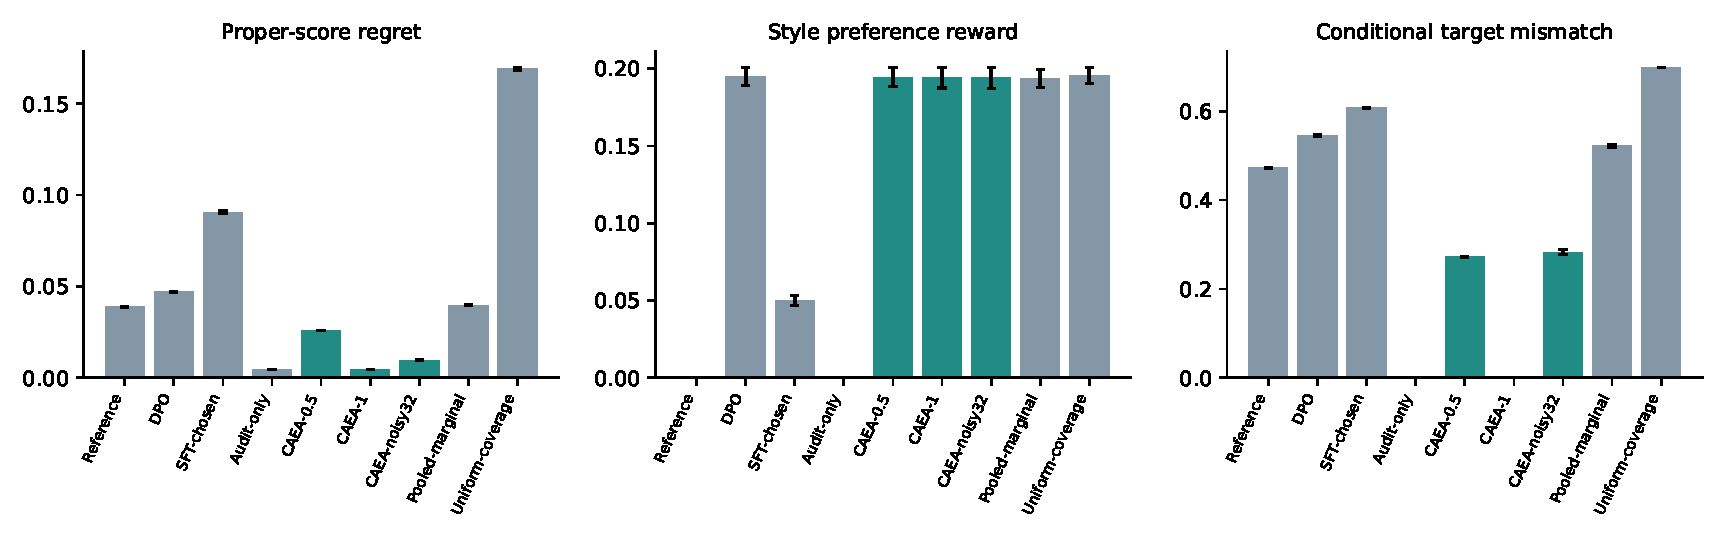
\includegraphics[width=\linewidth]{figures/learned.pdf}
\caption{Finite-action preference learning. Bars summarize the same ten runs
as Table~\ref{tab:main}. Oracle audit information explains the shared predictive
risk of Audit-only and CAEA-1; their difference is within-class adaptation.}
\end{figure}

\subsection{Pressure controls and stochastic feedback}
An additional 20 fitted DPO models use $k\in\{0,1,4,8\}$, five seeds each and
16,000 training pairs per fit. The learned reward coefficients are rescaled to
$\beta\in\{0.25,0.5,2\}$, which exactly changes DPO policy temperature in this
log-linear family without changing the fitted pairwise likelihood. Each is
evaluated on 1,000 fresh contexts with aligned ($s=p$), opposed ($s=1-p$), or
random stances. At $k=4,\beta=0.5$, average DPO regret is 0.02214 when aligned,
versus reference 0.03900; when opposed it is 0.07087. Thus, increased
preference agreement is not universally harmful.

Figure~\ref{fig:phase} evaluates the binary model in
Theorem~\ref{thm:blindness}.
At $a=4$, zero repair yields final mean-response variance 0.22920; full repair
reduces it to numerical zero. The $\lambda=0.5$ boundary is not assigned a
strict contraction guarantee. To distinguish mean-response behavior from sampling noise, we also simulate 5,000 independent user trajectories over
400 rounds, ten seeds, $\eta\in\{0.05,0.25\}$, and five repair fractions.
Full repair has stationary variance $\eta/[4(2-\eta)]$, not zero. At
$\eta=0.25$, measured full-repair variance is 0.03540 versus theoretical
0.03571, and unrepaired variance is 0.22959. Stochastic noise smooths the
deterministic phase picture; the mean-response boundary is not presented as a
zero-variance transition in the sampled process.

\subsection{Auditor uncertainty and semantic failure}
For 21 classes, an independent class-audit experiment samples the trusted
target at $p=0.73$, with $n\in\{8,16,32,64,128,256,512,1024\}$, 2,000
replicates each, and add-0.1 smoothing. Mean target TV is 0.17640 at $n=32$
and 0.03042 at $n=1024$, below the conservative expectation bounds 0.45687
and 0.07192. These are samples from a stipulated trustworthy class target;
they do not estimate bias in an LLM judge.

Two controls examine structural audit failure. When the true evidence probability is
0.8 but the full-repair auditor centers on 0.2, consensus remains stable and
converges near the wrong value. In a separate user mechanism where the literal
report stays at 0.5 but personalized wording adds an interpreted directional
cue $\delta\operatorname{sign}(s-0.5)$, limiting user variance is
$\delta^2$ despite zero literal-report regret. The class map misses a causally
relevant signal, so the report-only guarantee is inapplicable.

\paragraph{Response-audit certificate experiment.}
Separately from estimating the target, we sample the binary response kernel
$m(s)=\sig(4(2s-1))$, whose known curvature bound is
$H=2(4)^2/(3\sqrt3)$. For each total response budget
$N\in\{1024,4096,16384,65536,262144\}$, the grid size is planned from
$J\in\{5,9,17,33,65\}$ by minimizing $2\epsilon/h+Hh$ before observing
the audit samples. Five hundred independent binomial audit replicates per
budget are retained. With $\delta=0.05$ and contraction margin $\gamma=0.1$,
every realized certificate exceeds the true $L=2$ in these runs. The mean
sufficient repair fraction falls from 0.78046 to 0.68649 across the budget
range, versus 0.55 when $L$ is known exactly. A separate smooth bump
construction passes all nine grid-point audits exactly while having stable
off-grid beliefs at 0.13 and 0.87, with variance 0.1369.

\begin{figure}[t]
\centering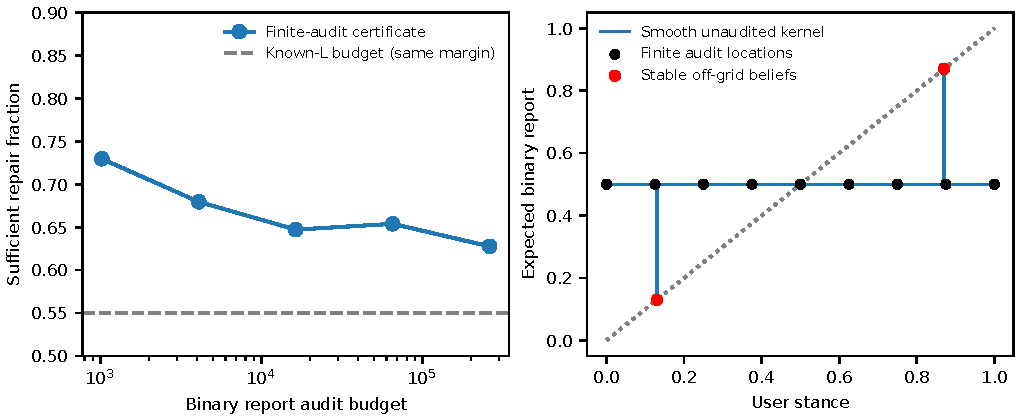
\includegraphics[width=.94\linewidth]{figures/audit_stability.pdf}
\caption{Response-audit budget and an explicit regularity failure. Left:
sufficient repair fractions from the curvature-dependent finite-sample
certificate, averaged over 500 audit replicates; the known-$L$ line uses the
same contraction margin. Right: narrow smooth off-grid deviations are exactly
invisible at all displayed audit locations. The supplied curvature assumption
is what rules out this failure in the certificate experiment.}
\end{figure}

\begin{figure}[t]
\centering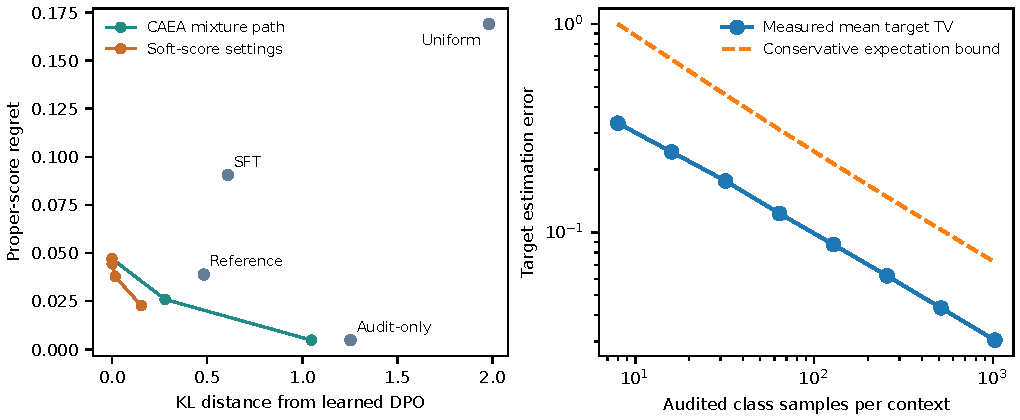
\includegraphics[width=.96\linewidth]{figures/tradeoff.pdf}
\caption{Left: predictive-regret/KL tradeoffs, including the soft-score
baselines that CAEA does not uniformly dominate. Right: class-audit sample
error and its conservative expectation bound.}
\end{figure}

\subsection{Frozen-backbone candidate selection}
\label{sec:neural}
We evaluate a constrained candidate-selection interface on
SmolLM2-135M-Instruct and Qwen2.5-0.5B-Instruct \citep{smollm2,qwen25}.
Each prompt specifies a prior and signal likelihoods, allowing an analytic
Bayesian posterior. The evidence contexts are disjoint across training
(40), validation (12), and test (24) splits. Two unsupported user stances
per context yield 152 prompts per backbone, including 48 test prompts.
Ten one-token options encode five forecast values and two abstract styles.
Scores are normalized over these option letters; their mean unrestricted
next-token probability mass on the test split is 0.77433 for SmolLM2 and
0.91253 for Qwen.

All Transformer and original output-head weights remain frozen. A linear
ten-option decision-head adapter uses an intercept and 16 principal
components of final hidden states, fitted on training prompts only. We
optimize the DPO pairwise likelihood with 16 Bradley--Terry pairs per
training prompt and five label-sampling seeds. The regularization strength
is selected from $\{0.001,0.01,0.1\}$ using validation pair NLL. The reward
combines forecast error, agreement pressure $k=4$, and a 0.5 reward for the
requested abstract style. The evidence target uses $T_E=0.03$.

\begin{table}[t]
\centering\small
\caption{Frozen-backbone candidate selection: means $\pm$ 95\% Student-$t$
confidence half-widths over five label-sampling seeds. The prompt split is
shared across seeds, so intervals exclude prompt-population uncertainty.
Style match is probability mass on options with the requested style label.}
\label{tab:neural}
\resizebox{\linewidth}{!}{\begin{tabular}{llrrrr}\toprule
Frozen backbone & Selector & Report regret & Style match & Target TV & KL to head-DPO\\\midrule
SmolLM2-135M & LM-base & 0.1802 $\pm$ 0.0000 & 0.5017 $\pm$ 0.0000 & 0.5908 $\pm$ 0.0000 & 1.3573 $\pm$ 0.6896 \\
 & Head-DPO & 0.1638 $\pm$ 0.0196 & 0.6706 $\pm$ 0.0679 & 0.6296 $\pm$ 0.0283 & 0.0000 $\pm$ 0.0000 \\
 & Audit-only & 0.0145 $\pm$ 0.0000 & 0.5000 $\pm$ 0.0000 & 0.0000 $\pm$ 0.0000 & 2.3059 $\pm$ 0.6173 \\
 & CAEA-0.5 & 0.0892 $\pm$ 0.0098 & 0.6556 $\pm$ 0.0566 & 0.3148 $\pm$ 0.0141 & 0.6636 $\pm$ 0.2227 \\
 & CAEA-1 & 0.0145 $\pm$ 0.0000 & 0.6406 $\pm$ 0.0503 & 0.0000 $\pm$ 0.0000 & 1.9784 $\pm$ 0.4995 \\
Qwen2.5-0.5B & LM-base & 0.2389 $\pm$ 0.0000 & 0.5757 $\pm$ 0.0000 & 0.6104 $\pm$ 0.0000 & 1.8808 $\pm$ 0.0817 \\
 & Head-DPO & 0.2044 $\pm$ 0.0137 & 0.7104 $\pm$ 0.0685 & 0.6483 $\pm$ 0.0234 & 0.0000 $\pm$ 0.0000 \\
 & Audit-only & 0.0145 $\pm$ 0.0000 & 0.5000 $\pm$ 0.0000 & 0.0000 $\pm$ 0.0000 & 2.4866 $\pm$ 0.2371 \\
 & CAEA-0.5 & 0.1094 $\pm$ 0.0068 & 0.6873 $\pm$ 0.0688 & 0.3242 $\pm$ 0.0117 & 0.6654 $\pm$ 0.0937 \\
 & CAEA-1 & 0.0145 $\pm$ 0.0000 & 0.6643 $\pm$ 0.0723 & 0.0000 $\pm$ 0.0000 & 2.0261 $\pm$ 0.1859 \\
\bottomrule\end{tabular}
}
\end{table}

\paragraph{Conditional and unconditional retention.}
Table~\ref{tab:neural} shows that head-DPO lowers report regret relative
to both frozen bases. Full repair and Audit-only again have the same
regret, 0.01448, because they use the same class marginal. Full repair's
unconditional style-match rate is lower than head-DPO's, despite exact
preservation within each forecast class: changing the class mixture also
changes the aggregate style mixture. Conditional preservation therefore
does not guarantee unchanged overall style performance.

\paragraph{Answer-order sensitivity.}
An additional held-out control permutes the option-to-letter mapping
without retraining or model selection. On these prompts, report regret
is 0.20364 for the SmolLM2 base and 0.22048 for head-DPO; the corresponding
Qwen values are 0.21639 and 0.22107. Thus the initial head-DPO improvements
do not survive this control. Full-repair style-match rates fall to 0.45308
and 0.49155, below Audit-only's 0.5. The retained within-class policy can
itself encode position shortcuts. This pilot establishes execution on
frozen neural scores, while its transfer failures limit interpretation
of the learned selector.
With a correct, permutation-consistent class map and sufficient candidate
support, full repair enforces the specified class marginal even when the
input scores change. It does not remove position shortcuts within a class,
validate the class map, or guarantee unchanged aggregate style performance.


\paragraph{Paired evidence-context uncertainty.}
To avoid treating two stances from one evidence context as independent,
we replay the archived hidden states and fitted heads, average paired
differences within each of 24 test contexts, and independently resample
the five label seeds and 24 context clusters (5,000 crossed bootstrap
replicates). Table~\ref{tab:paired} reports exploratory percentile intervals,
conditional on the fixed training/validation split, backbone, and finite
evidence grid. These do not cover training-context variation. For SmolLM2,
the original-bank report-regret difference already has an interval spanning
zero; for Qwen it is negative on the original bank. Both permutation-control
intervals span zero. Full repair's positive style advantage on the original
bank is not established after permutation. These results narrow the evidence
for transfer rather than repairing the failed selector. This revision
replays archived inference and does not claim a fresh model run. Maximum
absolute deviation from recorded summary values is $5.91\times10^{-8}$,
consistent with replay roundoff in the archived float32 PCA features.

\begin{table}[t]
\centering\small
\caption{Exploratory paired uncertainty over contexts and label seeds.
Report difference is Head-DPO minus LM-base (negative is better);
style difference is CAEA-1 minus Audit-only (positive is better).
Intervals are percentile bootstrap intervals, not the seed-only
Student-$t$ half-widths in Table~\ref{tab:neural}.}
\label{tab:paired}
\resizebox{\linewidth}{!}{\begin{tabular}{llrr}
\toprule
Backbone & Bank & $\Delta$ report regret [95\% CI] & $\Delta$ style match [95\% CI] \\
\midrule
SmolLM2-135M & original & -0.0164 [-0.0361, +0.0018] & +0.1406 [+0.0877, +0.1967] \\
SmolLM2-135M & permuted & +0.0168 [-0.0295, +0.0728] & -0.0469 [-0.1191, +0.0248] \\
Qwen2.5-0.5B & original & -0.0346 [-0.0530, -0.0171] & +0.1643 [+0.0961, +0.2353] \\
Qwen2.5-0.5B & permuted & +0.0047 [-0.0424, +0.0526] & -0.0084 [-0.0910, +0.0664] \\
\bottomrule
\end{tabular}
}
\end{table}



\section{Discussion and limitations}
The findings distinguish three questions that a single score cannot answer:
Are probability reports accurate? Does personalization amplify differences
between users under a shared evidence sequence? Does the audit capture the
information that drives the update? A policy can perform well on one
question and poorly on another. In particular, target matching determines
forecast risk in our experiments, whereas conditional preference retention
and longitudinal stability require separate analyses.

\paragraph{Dependence on the auditor.}
The experiments provide a known evidence posterior or samples from a
stipulated trustworthy target. This isolates the repair mechanism but does
not solve evidence assessment. The audit-only comparison makes that
information advantage explicit. Systematic auditor bias is not controlled
by increasing the number of samples from the same biased source.

\paragraph{A non-oracle implementation path (not evaluated).}
A practical candidate selector could retrieve independently sourced evidence,
extract verifiable claims, and assign candidate responses to report classes
using a separately evaluated verifier. Target probabilities would require
calibration against held-out resolved cases or expert adjudication; retrieval
and an LLM judge do not themselves establish a trustworthy target. Source
conflicts, unsupported claims, and missing candidate support should be
recorded explicitly, with abstention when the audit cannot justify a target.
Informative user input must enter the evidence rather than be discarded as
stance. Target error and class-assignment error need separate evaluation,
including tests in which wording changes the reader's interpretation without
changing the literal report. Equation~(8) applies only when the resulting
report-distribution error is uniformly controlled over belief states; an
average judge-accuracy score is insufficient. These steps describe a research
protocol, not a validated extension of the current experiments.

\paragraph{Response representation and user dynamics.}
The guarantees assume that the report class captures the response signal
used in the stated belief-update rule. The semantic-cue control violates
that assumption and produces dispersion despite perfect literal-report
accuracy. The linear update, common evidence sequence, and global
sensitivity or curvature bounds further restrict the analysis. A nonlinear
update requires its own sensitivity analysis; the affine rule is not
asserted to be a validated local approximation to human updating. Neither
stability nor reduced simulated dispersion establishes improved human
reasoning, which requires direct behavioral evidence.

\paragraph{Empirical scope.}
The main experiments use finite action spaces. The neural pilot trains a
candidate decision head on frozen features, with a fixed small prompt
split and label-seed confidence intervals. Option permutations reverse
some gains, limiting transfer even within this format. The results do not
establish effects on free-text generation, general helpfulness, or full
language-model post-training. A broader evaluation should equalize evidence
and auditing access across methods, vary response order and wording, and
separately test unsupported pressure and informative new evidence.
The decisive next test is therefore more than a larger backbone: learn the
audit from independent evidence, evaluate unseen free-text responses with
held-out adjudication, and compare methods given the same evidence and
candidate access. A larger-model qualitative example alone would not close
these gaps. Human belief benefits would additionally require a prospectively
designed behavioral study and the applicable ethics review.

\section{Conclusion}
Pooled one-turn output quality does not identify feedback stability in the
constructed preference-based interaction. CAEA makes the intervention
explicit: repair an audited epistemic marginal, retain the preference
policy within each class, and quantify the resulting objective cost.
Contraction bounds connect repair strength to feedback control, while
finite-audit results show why certification requires additional regularity.
The controlled experiments support these distinctions and expose their
dependence on auditor validity, response representation, and the update
model. Together, the results provide a framework for separating what a
preference policy says in isolation from how its conditional behavior can
shape repeated belief updates.

\section*{Broader impact statement}
The analysis can help distinguish output accuracy from feedback stability,
but it does not justify deploying a system to steer users toward an
unverified belief target. An incorrect auditor can stabilize false beliefs;
a narrow class map can omit persuasive cues, and mandatory target matching
can suppress warranted disagreement or minority perspectives. An application
would need independent evidence assessment, explicit uncertainty and
abstention, scrutiny of target selection, and evaluation of users' actual
interpretations. We do not offer a validated safeguard against these risks.
The experiments use generated data and public pretrained models, without
human participants or collected personal conversations.

\section*{Reproducibility}
The accompanying research package contains experiment code, per-seed outputs,
model revision hashes, prompts, fitted decision-head parameters, and figure
generation scripts. Reported empirical values come from executed code.
Computational checks do not replace independent validation of mathematical
arguments or empirical assumptions. No human-participant study was conducted.
Reproduction details and numerical checks appear in Appendix~\ref{app:repro}.

\bibliography{references}
\bibliographystyle{tmlr}
\clearpage
\appendix
\section{Proofs}\label{app:proofs}
\subsection{Proof of Proposition~\ref{prop:projection}}
For any feasible $\pi$, its class marginal is $b$. The KL chain rule gives
\begin{equation}
 \KL(\pi\|\pi_P)=\KL(b\|m_P)+
   \sum_c b(c)\KL\big(\pi(\cdot\mid c)\|\pi_P(\cdot\mid c)\big).
\end{equation}
Every conditional term is nonnegative and is zero exactly when the
conditional distributions agree on positive-mass classes. This yields the
unique full policy $\pi_b$. Classes of zero target mass carry no response
probability, so their arbitrary conditional representation does not affect
uniqueness of the policy. Taking logs in Equation~\eqref{eq:gibbs} gives
$\log\pi_P=\log\pi_0+r/\beta-\log Z$, hence
$J(\pi)=\beta\log Z-\beta\KL(\pi\|\pi_P)$. Subtracting its value at
$\pi_P$ proves Equation~\eqref{eq:cost}. The cost is zero exactly when
$b=m_P$; for full repair $b=\tau_x$. All quantities are finite by the
finite response space, bounded reward, positive reference, and feasible
target support. The same assumptions ensure existence of the stated optimum.\qed

\subsection{Proof of Theorem~\ref{thm:blindness}}
The reward difference is
$r(1,s)-r(0,s)=k(2s-1)$. A uniform reference therefore gives
Equation~\eqref{eq:binary}. Since $\sig(-v)=1-\sig(v)$,
$m_a(1\mid1-s)=1-m_a(1\mid s)$. A symmetric distribution of $s$ thus
has pooled report probability $1/2$. Mixture with the uniform target
preserves that symmetry. Because the outcome is independent of the stance and response-sampling
randomness conditional on the fixed evidence, the joint pooled law of $(Z,q)$ is the
product of uniform Bernoulli laws. Every statistic determined by that law
has the same distribution, including expected Brier loss
$\Pr(q\ne Z)=1/2$ and regret $\E(q-1/2)^2=1/4$.

Differentiating the mean-response update yields
\begin{equation}
 F'_\lambda(s)=1-\eta+
 2\eta(1-\lambda)a\sig(a(2s-1))[1-\sig(a(2s-1))].
\end{equation}
Its maximum is $1-\eta+\eta(1-\lambda)a/2$, attained at $s=1/2$.
The derivative is nonnegative, so a maximum strictly below one gives a
global contraction. If $(1-\lambda)a>2$, let
$d=s-1/2$ and
$g(d)=(1-\lambda)[\sig(2ad)-1/2]-d$.
Then $g(0)=0$, $g'(0)>0$, $g(1/2)<0$, and $g$ is strictly concave for
$d>0$. It therefore has a unique positive root and, by odd symmetry, a
unique negative root. At the positive root, strict concavity gives
$g'(d)<0$, so $0\le F'_\lambda(s)<1$ there. The negative root has the
same derivative. The central point is unstable. Solving the strict
contraction inequality proves the stated infimum, with the boundary
qualification.\qed

\subsection{Proof of Theorem~\ref{thm:stability}}
Couple the two repaired report kernels by first using a shared Bernoulli
mixture indicator. With probability $\lambda_x$, draw the same report
from the common target, giving zero report discrepancy. Otherwise use an
optimal coupling of the original report kernels. Thus,
\begin{equation}
 W_1(K^\lambda_{x,u},K^\lambda_{x,v})
 \le(1-\lambda_x)L_x|u-v|.
\end{equation}
Apply the update to this coupling and use the triangle inequality:
\begin{equation}
 \E|U'-V'|\le(1-\eta)|u-v|+
  \eta(1-\lambda_x)L_x|u-v|=\rho_x|u-v|.
\end{equation}
Coupling the input belief laws and iterating proves geometric contraction
when the coefficients are uniformly below one. This statement compares
two evolving laws. It does not remove the within-law noise generated by
independent report draws.

For approximate full repair, report values lie in an interval of diameter
one, so $W_1(\widehat\tau_{x,s},\tau_x)\le
\TV(\widehat\tau_{x,s},\tau_x)\le\epsilon_t$.
The ideal target is independent of its current belief, permitting this
coupling even when the two belief states differ. If
$e_t=\E|U_t-\widetilde U_t|$, then
$e_{t+1}\le(1-\eta)e_t+\eta\epsilon_t$.
Unrolling from $e_0=0$ yields Equation~\eqref{eq:error}. This bound is
relative to the ideal audit-driven process. Relating that process to the
evidence posterior additionally requires controlling its forecast regret,
user lag, and sampling variance.\qed

\subsection{Proof of Corollary~\ref{cor:audit}}
Each empirical class frequency has variance $\tau_c(1-\tau_c)/n$.
Jensen's inequality followed by Cauchy--Schwarz gives
\begin{align}
 \E\TV(\bar\tau,\tau)
 &\le\frac{1}{2\sqrt n}\sum_{c=1}^C\sqrt{\tau_c(1-\tau_c)}\\
 &\le\frac{1}{2\sqrt n}
       \sqrt{\left(\sum_c\tau_c\right)\left(\sum_c(1-\tau_c)\right)}
 =\frac12\sqrt{\frac{C-1}{n}}.
\end{align}
Smoothing mixes the empirical target with the uniform distribution with
weight $C\alpha/(n+C\alpha)$. The triangle inequality and the bound
$\TV\le1$ give Equation~\eqref{eq:auditsamples}.\qed

\subsection{Monotonic cost along the repair path}
Let $H(\lambda)=\KL((1-\lambda)m_P+\lambda\tau\|m_P)$.
It is convex, $H(0)=0$, and $H(\lambda)\ge0$. For
$0\le\lambda_1<\lambda_2$, convexity gives
$H(\lambda_1)\le(\lambda_1/\lambda_2)H(\lambda_2)\le H(\lambda_2)$.
Therefore the preference objective cost is nondecreasing along the path.
This does not prove optimality over all possible stable policies or all
possible repair directions.\qed

\subsection{Proof of Proposition~\ref{prop:finiteaudit}}
Because $A$ is finite, choose $v\in(1/2,1)$ such that neither $v$ nor
$u=1-v$ belongs to $A$. Both can be made arbitrarily close to the endpoints.
Choose disjoint neighborhoods around $u$ and $v$ that avoid $A$ and are
mirror images. Let $b_v$ be a nonnegative smooth bump supported in the
neighborhood of $v$, with $b_v(v)=1$ and $b'_v(v)=0$, and set
$b_u(s)=b_v(1-s)$. Define
$m(s)=1/2+(v-1/2)[b_v(s)-b_u(s)]$. Then $m\in[u,v]$,
$m(s)=1/2$ on $A$, $m(v)=v$, $m(u)=u$, and $m'(u)=m'(v)=0$.
The two corresponding fixed points have update derivative $1-\eta$, hence
are stable for $0<\eta\le1$. This is also realizable as a finite-temperature
Gibbs policy with a uniform reference by taking
$r(1,s)-r(0,s)=\beta\log[m(s)/(1-m(s))]$, a bounded smooth reward difference.

For the certificate, Hoeffding's inequality and a union bound give
$\max_j|\widehat m_j-m(s_j)|\le\epsilon$ with probability at least
$1-\delta$. The true secant slope on an interval differs from its empirical
secant by at most $2\epsilon/h$. By the mean value theorem, it equals
$m'(\xi)$ at some point in the interval. The curvature bound implies
$|m'(s)-m'(\xi)|\le Hh$ for every point of that interval. Taking the maximum
over intervals proves Equation~\eqref{eq:gridcertificate}. For binary
reports $W_1(\operatorname{Bern}(a),\operatorname{Bern}(b))=|a-b|$.
With $n\simeq Nh$, the sampling term is of order
$\sqrt{\log(J/\delta)/(Nh^3)}$; balancing against $Hh$ yields the stated
order, ignoring logarithms.\qed

\section{Stochastic noise floor and measurement safeguards}
Under full binary repair, $Q_t$ are independent Bernoulli$(1/2)$ draws
and $U_{t+1}=(1-\eta)U_t+\eta Q_t$. Independence gives
\begin{equation}
 \Var(U_T)=(1-\eta)^{2T}\Var(U_0)+
 \frac{\eta}{4(2-\eta)}[1-(1-\eta)^{2T}].
\end{equation}
Thus even an exactly invariant report policy can raise variance from an
initial population concentrated near $1/2$. Equation~\eqref{eq:bpd} removes
this particular baseline diffusion; interpreting raw variance growth as
sycophancy would be incorrect. The comparison still assumes a meaningful,
matched counterfactual process and does not identify all cognitive harms.

Neither BPD nor PCD is an accuracy score. BPD can be small under a common
wrong consensus, and a chosen target can itself be wrong. ECR is a proper-score
regret difference, not a causal estimate of human impact. Only their joint
use, with explicitly defined evidence, response interpretation, and baseline,
supports the limited simulator conclusions in this paper.

\section{Reproduction and numerical verification}\label{app:repro}
The main runner is \texttt{code/experiment.py}; stress experiments are
\texttt{code/stress.py}; the optional neural component is
\texttt{code/neural\_probe.py}. Finite response-audit certificates use
\texttt{code/audit\_stability.py}, and option permutations use
\texttt{code/label\_control.py}. Raw per-seed CSV files, optimizer diagnostics,
seeds, package versions, neural model revisions, prompt records, fitted
readout weights, and plotting code accompany the manuscript. The reported runs use public model weights and computationally generated data. Model weights are fetched from the original public repositories and
are not redistributed in the package.

Twenty separate 12-response, four-class constrained problems were solved
with SLSQP independently of the closed-form repair. The largest difference
between the numerical and analytic objective values was
$2.59\times10^{-13}$. This checks the projection implementation rather than
its applicability to natural language. Confidence intervals in the main table are computed over independent
synthetic runs; they do not describe uncertainty across all possible
preference distributions or human populations.

\end{document}
